\documentclass[conference]{IEEEtran}
\IEEEoverridecommandlockouts
% The preceding line is only needed to identify funding in the first footnote. If that is unneeded, please comment it out.

\usepackage{amsmath,amssymb,amsfonts}
\usepackage{algorithmic}
\usepackage{graphicx} 
\usepackage{textcomp}
\usepackage{xcolor} 
\usepackage[backend=biber]{biblatex}
\addbibresource{main.bib}

\def\BibTeX{{\rm B\kern-.05em{\sc i\kern-.025em b}\kern-.08em
		T\kern-.1667em\lower.7ex\hbox{E}\kern-.125emX}}

\begin{document}
	
	
	\title{Earth at night*\\
		{\footnotesize \textsuperscript{*}The visualisation of average radiance in specific area}
	}

		\IEEEauthorblockN{4\textsuperscript{th} Wenjie Tong}
		\IEEEauthorblockA{\textit{Faculty of Computer Sciences} \\
			\textit{The University of Waikato}\\
			Guizhou, China \\
			benji.tong1117@gmail.com}

	} 
	
	\maketitle
	
	
	
	\subsection{Open Nighttime Lights}
	
	\subsubsection{Overview}
World Bank Light---Every Night is a comprehensive data repository of light satellite images collected at night by two sensors for the past 30 years: National Defense Meteorological Satellite Program (DMSP) Line of Business Scanning System (OLS), data from 1992 to 2017.
Visible infrared imaging radiometer suite (VIIRS) day and night band (DNB) data are 2012-2020.

Both DMSP-OLS and VIIRS-DNB sensors capture various low-light emission sources from the earth as optical data. These light source data mainly include brightness data generated by various human activities, such as city lights, gas flares, fishing boats, and agricultural fires, and also capture other natural light phenomena at night, such as aurora. The data repository is released and can be used for analysis. The data repository was established by the World Bank in cooperation with the National Oceanic and Atmospheric Administration (NOAA) and the University of Michigan. Most of the basic data come from the NOAA National Environmental Information Center ( NCEI) file.

After continuous exploration, development, updates, and upgrades, the University of Michigan’s additional processing supports access in cloud-optimized GeoTIFF format (COG) and searches using Spatio-temporal Asset Catalog (STAC) standards. The ever-improving standards facilitate the analysis and become part of the ready data ecosystem, which is improving access to geospatial data sets, which makes it more widely accepted by the public and can be easily discovered, processed, and analyzed Geospatial data. Our project data will also use cloud-optimized GeoTIFF format (COG) and STAC standards to implement network-level applications.


	\subsubsection{Remote sensing}
Research by NASA shows that modern remote sensing technology began with the invention of the camera more than 150 years ago. The first original photo appeared as a "still image", but it inspired people's ideas and practices for shooting and looking down on the surface of the earth. This idea appeared in the 1840s. The first photos were used for topographic mapping. Later in the First World War, the cameras mounted on the aircraft provided a bird's-eye view of a considerable surface area and provided a large amount of terrain data for military activities. After continuous research and development, the current remote sensing technology has reached a qualitative leap. It is now commonly used to describe the science and art of identifying, observing, and measuring objects without directly touching them. The process involves detecting and measuring radiation of different wavelengths reflected or emitted from distant objects or materials, through which they can be identified and classified by category/type, substance, and spatial distribution (NASA,2021, August 28).

\small 
{\bf 2.1 Orbits\rm} 
\\
{\bf 2.1.1 Polar and non-polar\rm}
Polar-orbiting satellites(fig3)are located in an orbital plane that is nearly 90 degrees inclined to the equatorial plane. This tilt allows the satellite to perceive the entire earth, including polar regions, to observe locations that are difficult to reach from the ground. Many polar-orbiting satellites are considered sun-synchronous, which means that the satellite passes through the same position at the same solar time in each cycle. The polar orbit can be ascending or descending. In an ascending orbit, the satellite moves from south to north as it passes the equator. In descending orbit, the satellite moves from north to south.

\usepackage{graphicx}

\begin{figure}[htbp]
	\centerline{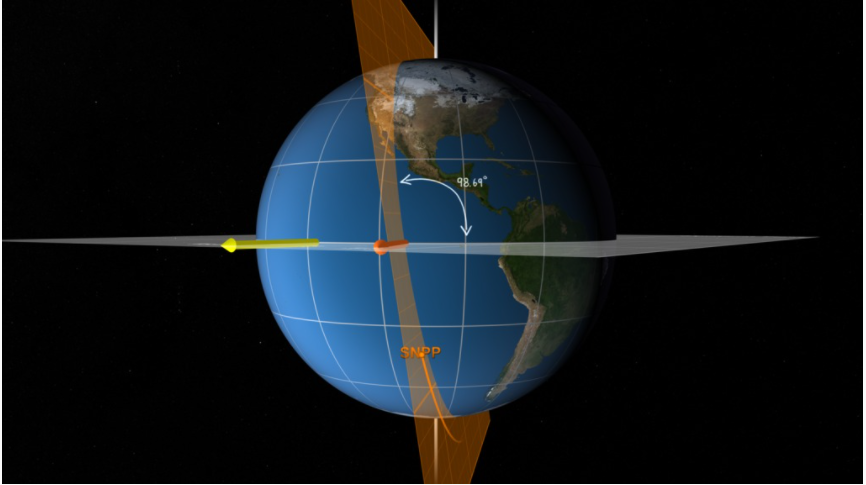
\includegraphics[width=260pt]{images/1.1.1.png}}
	\caption{Architecture}
	\label{fig3}
\end{figure}
 
\\
{\bf 2.1.2	Low-Earth orbit\rm}
Low Earth Orbit (LEO) is an orbit relatively close to the surface of the earth. It is usually located at an altitude of fewer than 2000 kilometers, but it may be as low as 400 kilometers above the earth. Compared to other orbits, it is low, but still far from the surface of the earth (NASA,2021, August 28).
It is the most commonly used orbit for satellite imaging because it is possible to take higher resolution images close to the surface. It is also the orbit used by the International Space Station (ISS) because it is easier for astronauts to travel to and from it at shorter distances. The satellite in this orbit travels at a speed of about 7.8 kilometers per second; at this speed, it takes about 90 minutes for the satellite to orbit the earth, which means that the International Space Station orbits the earth about 16 times a day (ESA, n.d.).
\begin{figure}[htbp]
	\centerline{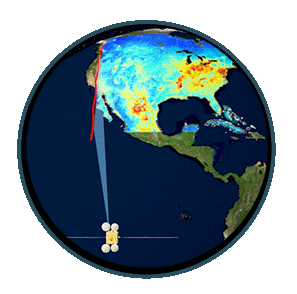
\includegraphics[width=260pt]{images/1.1.2.png}}
	\caption{Architecture}
	\label{fig3}
\end{figure}

\\
{\bf 2.1.3	Geostationary\rm}
The orbit of a geostationary satellite can only be achieved at an altitude very close to 35,786 kilometers, and the satellite can be fixed at one longitude of the equator. There are hundreds of communication satellites and several weather satellites in such orbits.

\begin{figure}[htbp]
	\centerline{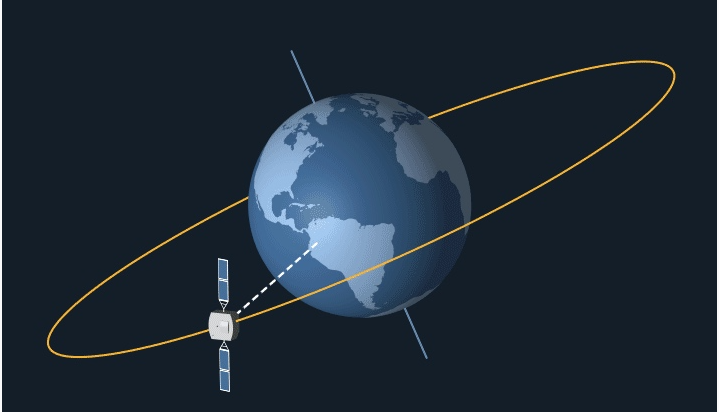
\includegraphics[width=260pt]{images/1.1.3.png}}
	\caption{Architecture}
	\label{fig3}
\end{figure}
\\


\small {\bf 2.2 Electromagnetic Spectrum\rm} 

\begin{figure}[htbp]
	\centerline{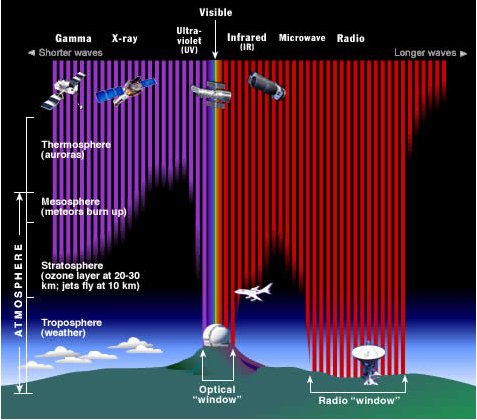
\includegraphics[width=260pt]{images/1.2.png}}
	\caption{Architecture}
	\label{fig3}
\end{figure}

{\bf 2.2.1	Radio\rm}

Very Low Frequency (VLF)
ELF is extremely low frequency and extremely low frequency, and its frequency is in the range of 300 Hz to 30 kHz. It is a kind of radio wave, just like AM/FM signal, but with a lower frequency. It is very useful because it is mainly reflected at a height of 60-90 kilometers in the D zone of the earth's ionosphere, so it is effectively guided to a global distance in the earth's ionospheric waveguide. It is widely used to set up radio receivers almost anywhere on the earth. This signal can receive short radiation from lightning strikes in half of the earth (Stanford VLF Group. n.d.).

Low Frequency (LF)
Low frequency refers to the radio frequency (RF) in the range of 30 kHz–300 kHz. Low-frequency AM broadcasting services are widely used in Northern Europe, North Africa, and Asia. In the current era, its main uses are aircraft beacons, navigation (LORAN), information, and weather systems. Numerous time signal stations such as MSF, DCF77, JJY, and WWVB are located in this frequency band, which is also called the kilometer band or kilometer wave (Low_frequency,n.d).

Medium Frequency (MF)
Medium Frequency means radio frequency (RF) in the range of 300 kHz to 3000 kHz. For example, the AM broadcast band is a medium wave (MW), and the MF band is also called the 100-meter band, which ranges from 100 to 1000 hundred meters (Medium_frequency,n.d).

High Frequency (HF)
The wave frequency of the high-frequency electromagnetic field is between 300 MHz and 3 GHz, and the wavelength is from 1 m to 10 cm. It is mainly human-generated non-ionizing electromagnetic radiation, which does not occur naturally in the environment, excluding low-amplitude VHF (Very high frequency) cosmic radiation. With the rapid development of wireless technology, HF is increasingly appearing in the environment.
\\
{\bf 2.2.2	Microwave\rm}
Very High Frequency (VHF)
Very high frequency (VHF) is ITU's electromagnetic wave in the range of 30 to 300 megahertz (MHz), and the corresponding wavelength is ten meters to one meter (Wikimedia Foundation. (2021, August 14).

Ultra-High Frequency (VHF)
Ultra-high frequency (UHF) is the ITU's 300 megahertz (MHz) and 3 gigahertz (GHz), also known as the decimeter band because the wavelength ranges from one meter to one-tenth of a meter. UHF radio waves propagate mainly through the line of sight; they can be blocked by various objects, and their transmission capacity will be limited by the blocking of objects. For example, TV broadcasting, mobile phones, GPS, WIFI, and walkie-talkies all use UHF to realize the dissemination and communication of data information (Wikimedia Foundation. (2021, August 8).

Super High Frequency (SHF)
The Super High Frequency (SHF) range is ITU to 3 to 30 gigahertz (GHz). This frequency belongs to the microwave band, so radio waves with these frequencies are called microwaves. There are many devices in this frequency range, such as radar transmitters, wireless local area networks, satellite communications, and it is also used in industrial microwave heating, medical diathermy, and microwave hyperthermia to treat cancer(Wikimedia Foundation,2021, July 15).

Extremely High Frequency (EHF)
Extremely high frequency (EHF) is a radio frequency in the electromagnetic spectrum from 30 to 300 gigahertz (GHz). Its frequency is between the ultra-high frequency band and the far-infrared frequency band, and below it is the terahertz frequency band. The wavelength of radio waves in this band varies from ten to one millimeter, so it is also called the millimeter-wave band and the radiation in its waveband is called millimeter waves (Wikimedia Foundation,2021, August 1).

\\         
{\bf 2.2.3	Infrared.\rm}
 Infrared radiation (IR) is a kind of radiant energy and electromagnetic radiation, which is invisible to humans, but we can still feel it. It occurs when atoms absorb and release energy with frequent fluctuations. All objects in the universe emit a certain degree of infrared radiation, such as the sun, fire, and the emergence of thermal imaging technologies are the research results of infrared technology (Lucas, J, 2019, February 27).
\\
{\bf 2.2.4	Visible\rm}
 The visible light spectrum is the segment of the electromagnetic spectrum that the human eye can view. Its wavelengths are 380 to 700 nanometers.
 The full spectrum of visible light can be divided into rainbow colors because each color has a different wavelength. Violet has the shortest wavelength, about 380 nanometers, and red has the longest wavelength, about 700 nanometers (NASA, n.d.).
 
\\
{\bf 2.2.5	Ultraviolet\rm}
UV (ultraviolet) light refers to the region of the electromagnetic spectrum between visible light and X-rays, with a wavelength between 400 and 10 nanometers. Among ultraviolet rays, red is the light with the longest wavelength, and violet is the light with the shortest wavelength. Therefore, the light with the longest wavelength is called infrared light, and the light with the shortest wavelength is called ultraviolet light (Stanford Solar Center, n.d.).
\\
{\bf 2.2.6	X-ray\rm}
X-rays are a penetrating form of high-energy electromagnetic radiation. The wavelength range of most X-rays is 10 picometers to 10 nanometers, the corresponding frequency range is 30 terahertz to 30 hertz (30×1015 Hz to 30×1018 Hz), and the energy range is 124 eV to 124 keV (Wikimedia Foundation. (2021, September 1).

\subsubsection{Spatial, spectral, and temporal resolutions in remote sensing}
	
\small {\bf 3.1 Spatial resolution\rm} 
\\
In remote sensing, the spatial resolution shows the smallest possible feature that a satellite image can display, which means that the size of a pixel on the ground constitutes the smallest "point" of an optical satellite image. If the satellite tries to capture the size of the scene 700KM from the earth (300m x 300m), the imaged pixels will be very low and the image will become very blurry (Muhebwa, A, nd). The spatial resolution is divided into 3 levels:
Low resolution: more than 60m/pixel
\\
Medium resolution: 10 ‒ 30m/pixel
\\
High resolution to ultra-high resolution: 30cm ‒ 5m/pixel
\\
Not many details about the capture are determined by the pixels of the spatial resolution. If improvements are made to obtain more captured details, a large number of cameras will be required to achieve detailed scenes. For the same purpose, space scientists need to use a single-pixel to represent the linear dimension on the ground, where the difference in pixels and colors will be recommended for measurements on the earth according to the satellite's use and coding method. In the 1980s, NASA satellite data from Landsat had 60 million pixels at the time, but with the advancement of the times and the rapid development of technology, 60 million pixels have become less leading. The current highest resolution satellites can provide 30 cm accurate imaging (EARTH OBSERVING SYSTEM,2021, August 2). 

\small {\bf 3.2 Spectral resolution\rm} 

The International Commission on Illumination (CIE) organization defines the light response of human vision as the range of 380nm to 780nm and provides a weight table so that the public can use the instrument to study the measured value at the wavelength multiplied by the corresponding human vision (Michael. (2021, June 21)). These tables are provided at intervals of 1 nanometer, 5 nanometers, and 10 nanometers. Resolution refers to how many data points are used in the calculation of the image. For the spectral resolution, it is to define the measurement point in the spectral result one step further.


\small {\bf 3.3	Temporal resolution\rm} 
Time resolution refers to the repetitive period or frequency at which the sensor revisits the same part of the earth's surface. Think of it as the time to take multiple measurements of the cross-section and then reconstruct the image. This time is also called the "revisit time" of the satellite. For example, the greater the stripe width of a polar-orbiting satellite, it is regarded as the width of the sensor's "cross-orbit" field of view during the passage of the orbit, and the higher the resolution time(Watson, N. J,2015).


	
	
	\subsection{Frontend}
	this is the explanation
	
	\subsection{Vue}
	this is the explanation
	
	\subsection{D3}
	this is the explanation
	
	\subsection{Spring-boot}
	Spring-boot is a Java web framework that can help developer build their web instance very quickly. It is easy to build a 
	stand-alone, production-grade application by it \cite{SpringBo66:online}. Because of its features such as no code generation 
	and no requirement for XML configuration, it is the best choose for a Java development team.
	
	\subsection{Oauth github}
	this is the explanation
	
	\subsection{Ansible}
	Ansible is a famous open source deployment platform, which is convenient to enable the infrastructure as code (IaC). 
	It is the main tool to deploy most of the services in this project. Especially, a single EC2 instance with public 
	IP is provided for it. But AWS service has to provision services by aws-cli instead of Ansible itself. There are still 
	some libaries providing these functions but mostly are from external part.
	
	\subsection{CloudFormation}
	CloudFormation is a service in AWS, which can organize services very quickly and configure them by yaml or json. There area
	several templates for provisioning different services. It is more convient than Ansible for some services. In this project, 
	RDS and Lambda Services are dependent on it.
	
	\subsection{Nginx/Tomcat}
	Nginx is the widely used web server all over the world. It also has the excellent performance as a reverse proxy. 
	Fontend server is the role in this project. Tomcat, which is behind Nginx, is a tranditional Java web container supporting 
	Java Servlet. The visualisation is deisgned by Java and run in this container. Both Nginx and Tomcat are well-known because of 
	the open source community and internet companies choosing.
	
	\subsection{RDS/Lambda/Secrets Manager/SQS/EC2/NAT}
	These items are names of services on AWS. Especially, Lambda are used to generate temperary password of RDS, and store it in 
	Secrets Manager. It is really a good method to enhance the security for the password of database. On the other hand, NAT is a 
	good feature for isolating the internal and external networks, but the price is too high to be used all the time in this project.
	
	\section{Proposed solution}
	
	A demo has finished all of tasks following the plan on time in this project. But to save budget, stoping NAT and processing parts of data are 
	the temporary approaches. It is also possible to deal with the cloud and other disruption to ensure the accrute radiance value. All the 
	other details are described as below.
	
	\subsection{Whole infrastructure}
	The main architecture is shown as Fig.~\ref{fig2}. First of all, two kinds of IaC platform, which are Ansible and CloudFormation.
	Ansible is the first choice that can be esily used in most of situations. When some service need to configure complicatedly, CloudFormation is 
	better. Secondly, NAT and ELB are the only entrance to the project. That is the best practice for network security that can mitigate the effects 
	of public cyberattacks. Thirdly, IAM roles are used at all kinds of important scenarios, for example, deployment, database visiting, various services visiting.
	
	The source code of entire demo was maintained on Github. The repository URL is https://github.com/A2Inc/A2. There are various languages in it including 
	CSS, Vue, Java, JavaScript, Python, Tex. The contributions of team on this demo are shown on Github as Fig.~\ref{fig3}.
	
	\begin{figure}[htbp]
		\centerline{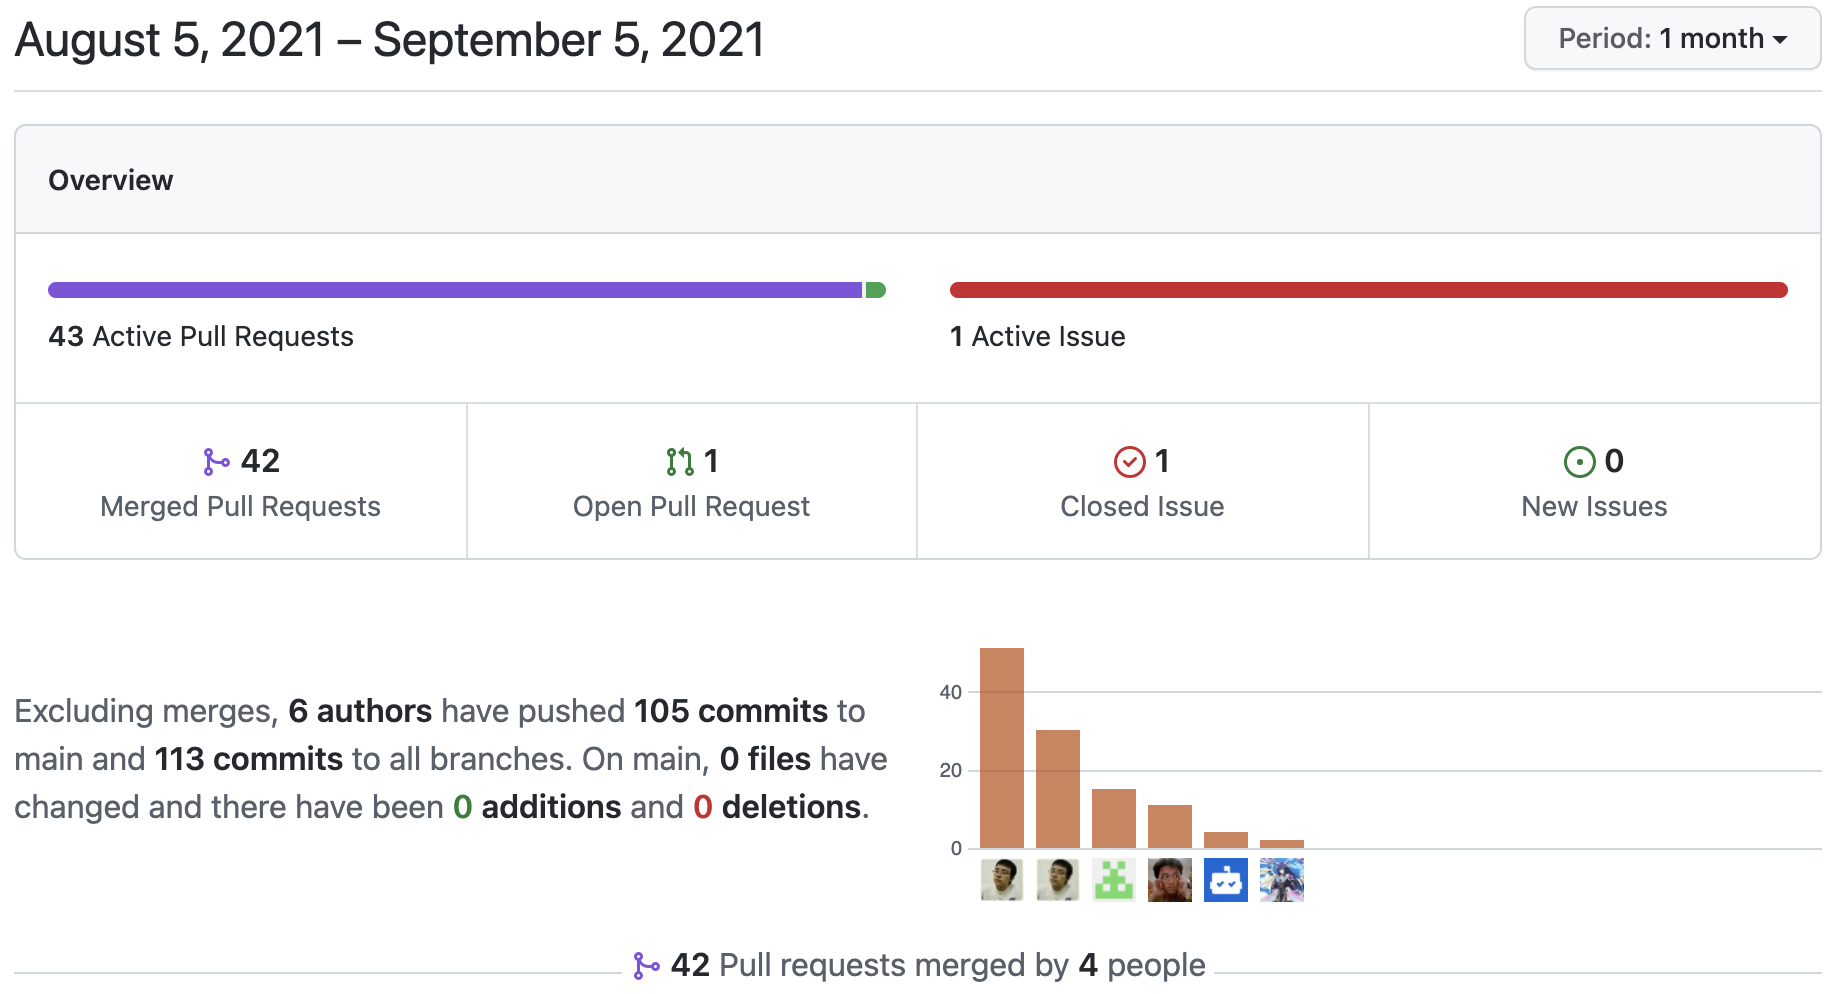
\includegraphics[width=260pt]{images/github.png}}
		\caption{Overview of Github}
		\label{fig3}
	\end{figure}
	
	Java, Python and Vue are the most useful tool in this demo. The reason of choosing Java is that almost all of the team members has been good at it. Python 
	has a lot of library processing images, so it is the best choice for geospatial imagery. Vue has powerful frontend capabilities, so it is the best for a 
	visualisation demo. Latex are used to generate the report and slides.
	
	\subsection{Frontend}
	
	\subsection{Login}
	
	\subsection{Data processing}
	\subsubsection{Data Overview}
    The Resources on AWS: 
	\keyword{Description}
	Light Every Night dataset of all VIIRS DNB and DMSP-OLS nighttime satellite data
	\keyword{Resource type}
	S3 Bucket
    \keyword{Amazon Resource Name (ARN)}	
	arn:aws:s3:::globalnightlight
	\keyword{AWS Region}
	us-east-1
	\keyword{AWS CLI Access (No AWS account required)}
	aws s3 ls s3://globalnightlight/ --no-sign-request
	For implementing the web-level application, understanding the database of the Light Every Night dataset is essential for our team. Then I have accessed this dataset via the AWS instance Linux server. 
	Under this path, there are three main types of folders, like-named by date (201204,201505…201603), named by satellites (F10, F12…F18), and named by npp_date.
	\subsubsection{DMSP-OLS}
	DMSP is a series of polar-orbiting satellites of the US Air Force. The sensors on this model satellite were used in the initial design to observe weather-related indicators in the visible and infrared wavelength ranges during the day and night. DMSP satellites can be divided into "day/night" or "dawn/dusk" satellites according to their transit time. One side of the orbit of the day and night satellite images the dayside of the earth, and the other side images the night side. In 1992, when the digital archive began to be created, two DMSP satellites collected data and named them F10 and F11. F10 is in day/night orbit, F11 is in dawn/dusk. Since then, eight satellites have been launched, F12-F19, of which F12, F14, F15, F16, and F18 were launched in day/night orbits.
	
	This part DMSP-OLS data which are named from DMSP satellites as I mentioned before. The file name was generated from the satellite's name and year. Like F101992, which means the data was collected by satellite F10 in 1992. There are many files from 1992 to 2013 that can be used by the public.
	\begin{figure}[htbp]
		\centerline{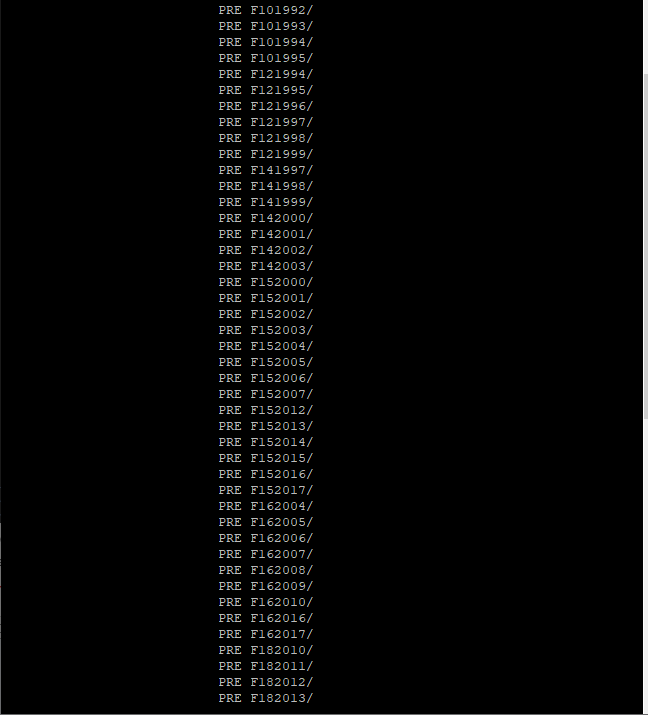
\includegraphics[width=260pt]{images/2.png}}
		\caption{Architecture}
		\label{fig3}
	\end{figure}
This picture is showing lots of folders of nighttime data.  In those folders, there are tons of.OIS files. 
For example: F12199501010014.night.OIS 
F12 -> satellite name
1995 -> year at start of orbital segment
01 -> month at start of orbital segment
01 -> day of month at start of orbital segment
00 -> hour of day at start of orbital segment
14 -> minute of hour at start of orbital segment
.night -> orbit is cropped to only nighttime data
.OIS -> acronym for OLS Interleaved Smooth
All those details about this file are giving more information for users to understand how the data be stored in the AWS database server. 

The satellite's timeline illustrates that the "F" satellites be used in different years.

	\begin{figure}[htbp]
	\centerline{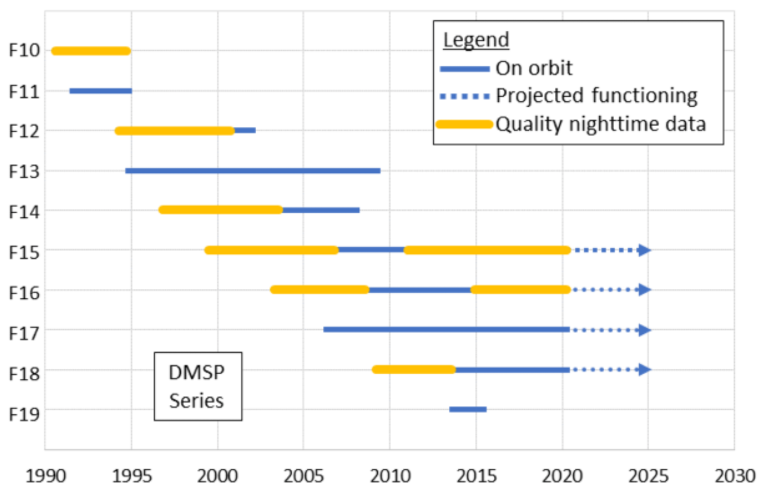
\includegraphics[width=260pt]{images/2.1.png}}
	\caption{Architecture}
	\label{fig3}
\end{figure}

The line chart demonstrates the different periods of how they are used in acquiring nighttime data.  It is clear to know F10 satellite is the first one which is used in collecting nighttime data in 1995. Then more and more satellites like F11, F12, F13, and F19 be created to take monitoring data missions.

\subsubsection{VIIRS-DNB: the follow-on sensor for the DMSP-OLS}
The follow-on sensor for the DMSP-OLS is called the VIIRS-DNB sensor, therefore there are many aspects of the VIIRS-DNB sensor that are the same as DMSP-OLS. Compared with DSMP-OLS, DNB is a scanning radiometer capable of low-light imaging and is launched on a sun-synchronous polar-orbiting platform. They regularly collect 14 orbits every day and image the earth during the day and night every 24 hours. According to the basic data of collection, they might look exactly the same but do more researches on nighttime data, almost all aspects of the DNB sensor itself are better than DSMP-OLS.

	\begin{figure}[htbp]
	\centerline{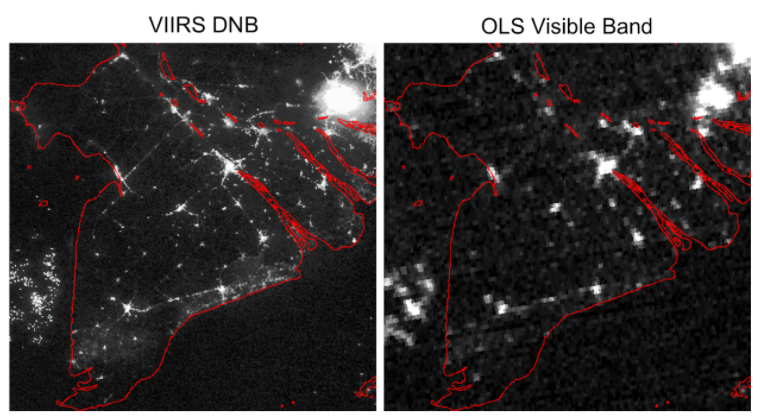
\includegraphics[width=260pt]{images/3.png}}
	\caption{Architecture}
	\label{fig3}
\end{figure}

The compared satellite pictures above show the different resolutions and details, and the result illustrates the VIIRS DNB's satellite data providing a clearer image.

In the AWS database, the folder includes massive files with NPP titles or names by date. 

\begin{figure*}[t]
	\subfloat[Figure 4\label{fig:4}]
	{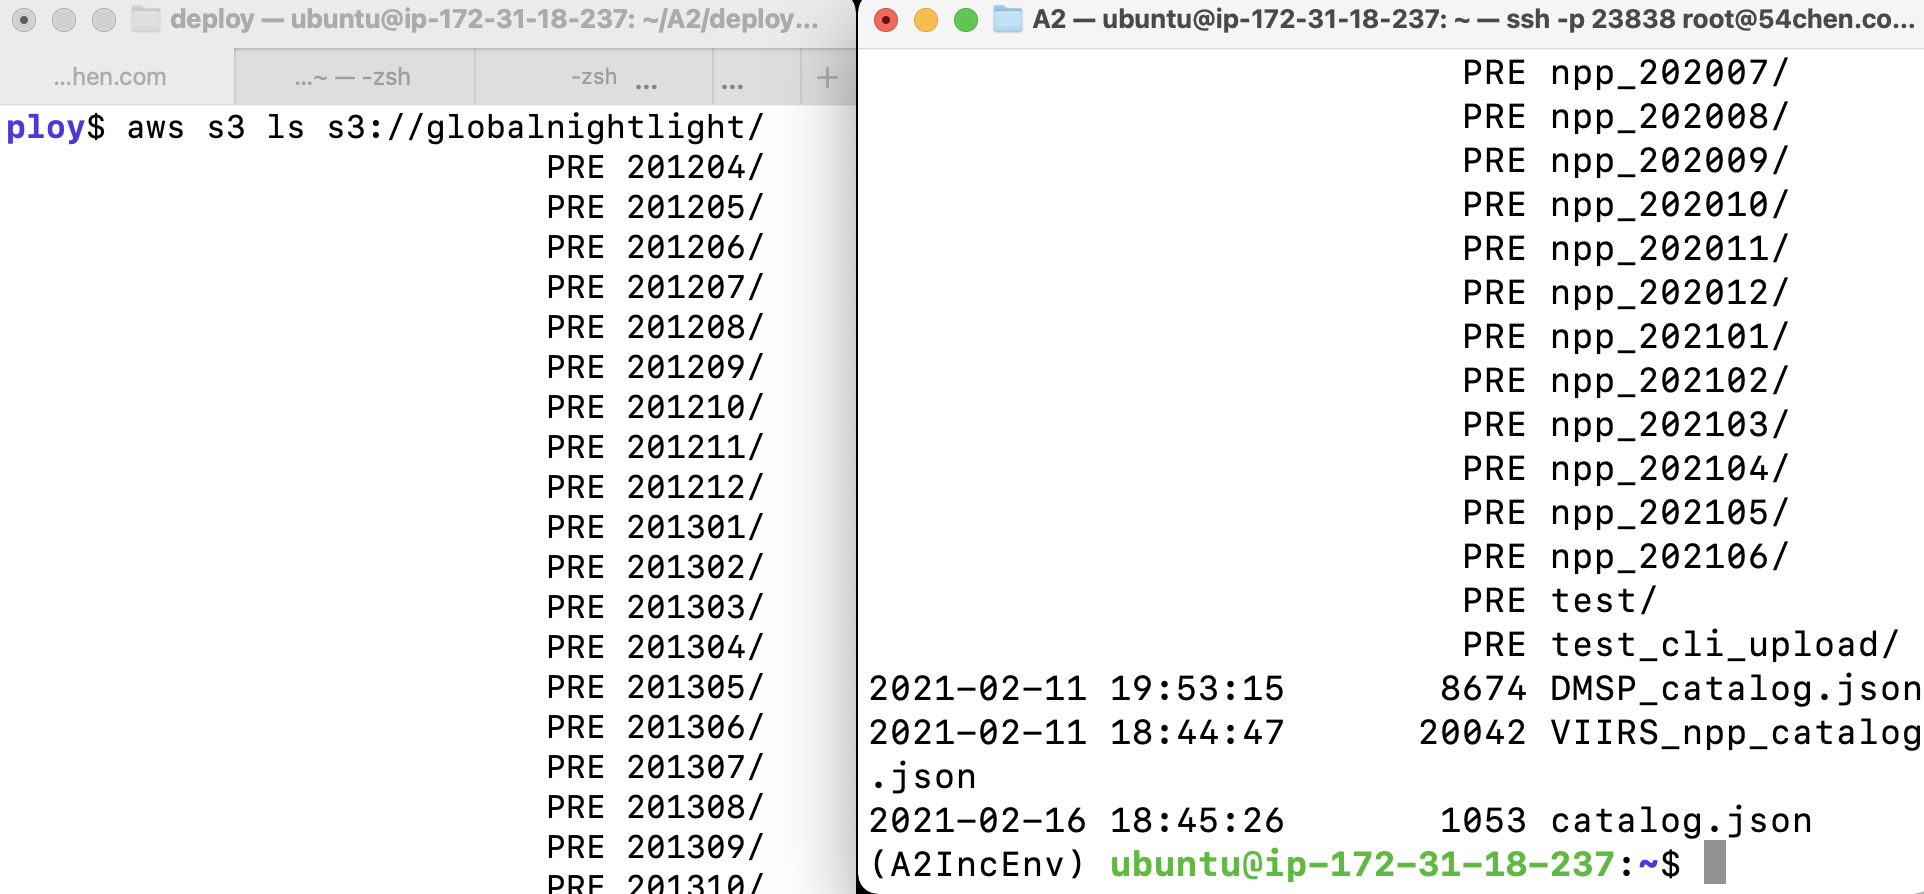
\includegraphics[width = 0.3\linewidth]{figs/3.1.png}} \quad
	\centering
	\subfloat[Figure 5a\label{fig:5a}]
	{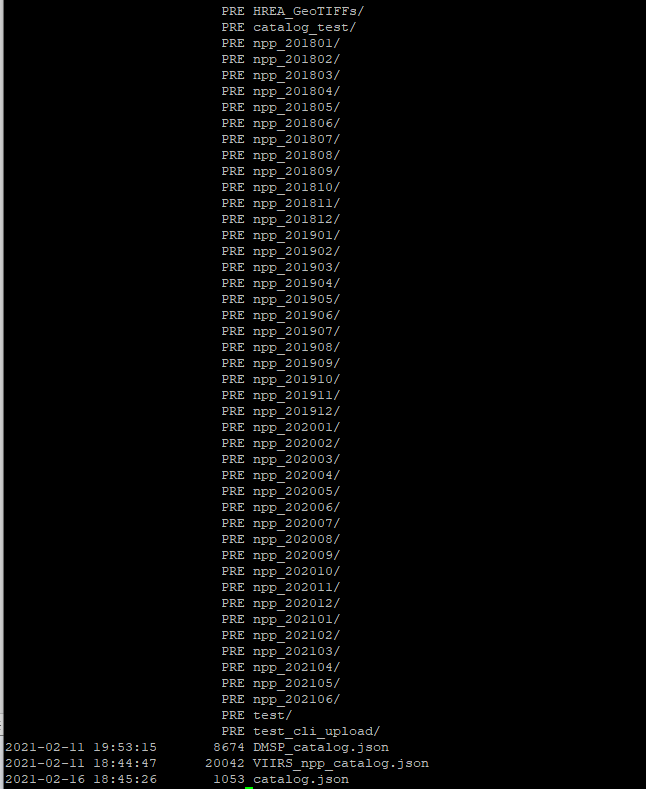
\includegraphics[width = 0.3\linewidth]{figs/3.2.png}}\quad
	\centering

\end{figure*}

The file named npp_year and month is because of the data collection from VIIRS-DNB( the following DMSP-OLS sensor). It has some difference between DMSP.
For example:
SVDNB_npp_d20150504_t1335358_e1341162_b18219_c20150504194116381040_noaa_ops.rade9.co.tif
The file structure is:\\
npp_d20150504_t1335358_e1341162_b18219\\
npp:satellite ID\\
d20150504: start date of first scan in aggregate (2015/05/04)\\
t1335358: time of first scan (13:35:35.8)\\
e1341162: time of last scan (13:41:16.2)\\
b18219: orbit number of first scan\\

SVDNB_npp_d20150504_t1335358_e1341162_b18219_c20150504194116381040_noaa_ops\\
SVDNB: Day/Night Band SDR (all possible product IDs are listed below)\\
npp_d20150504_t1335358_e1341162_b18219: aggregate identifier\\
C20150504194116381040: creation date/time of SDR\\
noaa:data origin\\
ops:data domain

\subsubsection{Data structure}
The geospatial data be collected by satellites then all data will be stored in different types of formats or data types. In our project, there are two types of data formats, Raster file, and Vector file.

\small {\bf 5.1 Raster file\rm} 
The raster image is an image file format, which is composed of a pixel matrix composed of multiple grids, and each pixel contains an information value. The change of this information value will be reflected in different colors, positions, and sizes. The most commonly used raster data, such as aerial photographs, satellite images, or elevation surfaces. These oversized pictures are taken and collected through the reflection of the spectrum. Moreover, today's raster images are usually .BMP, .GIF, .JPEG, .PNG and .TIFF files (Katie, 2020, May 8). At present, almost all the images that the public can see on the Internet and the images taken by digital cameras are raster images. In our project, TIFF data files will become our research object.
{\bf Use raster as the base map\rm}
In GIS, raster data is usually used as the background display screen of other feature layers. Such layers are orthophotos, which not only provide additional information but also make map users more confident that the map layers are spatially aligned and represent actual objects. There are three main sources of such images, namely orthophoto aerial photography, orthophoto satellite images, and orthophoto scanned maps (ArcGIS for Desktop, (n.d.).

{\bf Use raster as a surface map\rm}
Rasters are usually used to represent data that changes continuously along the surface, such as rainfall, temperature, density, etc. The map draws the surface of the map through the continuously changing data of countless small grids. The continuous change of grid color reflects the change of a region at present or within a period (ArcGIS for Desktop, (n.d.).

{\bf 5.2 Vector file\rm}
In our project, the vector format data is not the main research object, but it is also a format that our team needs to understand. A vector data file is an image that can be scaled to any size without losing its quality and clarity. Changing the file has an advantage because its scaling depends on mathematical equations. This vector file is more flexible and has perfect image quality. Compared with Raster files, pixilation will not lose sharpness when zooming in, and raster graphics will be greatly affected to form sharp contrasts (Logogenie.net,n.d.).


\subsubsection{GeoTIFFs & Cloud-optimized geoTIFFs (COGs)}
Most of the files in the data on the AWS server are TIFF or TIF files, and these files are a file format used to store raster files. GeoTIFF is a TIFF file that follows specific standards used to construct metadata, such as geographic reference information, spatial extent, resolution, and number of layers.
Cloud Optimization GeoTIFFs (COG) is a cloud-optimized file viewing, reading, and usage solution. The OGC GeoTIFF standard is the OGC implementation standard(NASA,2021, September 8). The files of GeoTIFFs are also GeoTIFF, and this data structured method allows users to query these files through Web services. However, this advantage allows users to query, analyze, visualize or download part of the COG file online without downloading the entire file. Such a database reading solution is also used by our team.

\subsubsection{Spatial-Temporal Asset Catalog (STAC) standard}
The SpatioTemporal Asset Catalog (STAC) specification provides a common language to describe a series of geospatial information in order to provide easier indexing and searching. A "space-time asset" is any file that represents information about the Earth captured in a specific space and time. The STAC specification is to allow all providers to publish new data sets or APIs without writing new code when they are published as a spatiotemporal asset catalog (SpatioTemporal Asset Catalog, n.d.). First of all, for providers, STAC is a standardized method for exposing Spatio-temporal data collections while cataloging assets and STAC is also a unified asset indexing method. Second, developers can build infrastructure to host, ingest, or manage spatial data collections, and can be extended to customize domains. Finally, data consumers often have to build a unique pipeline for each different data set they use.


	The pictures in S3 are based on two essential formats, which is STAC and COG. The satellites generate them everyday. World Bank organized the global night lights project 
	to store these files in S3. When it comes to deal with the satellite imagery, Python has a lot of easy libraries for geospatial calculating. GDAL is the most useful one. 
	It is integrated with Python very well, and is very good at reading and writing raster or vector geospatial file formats.
	
	
	\begin{figure}[htbp]
		\centerline{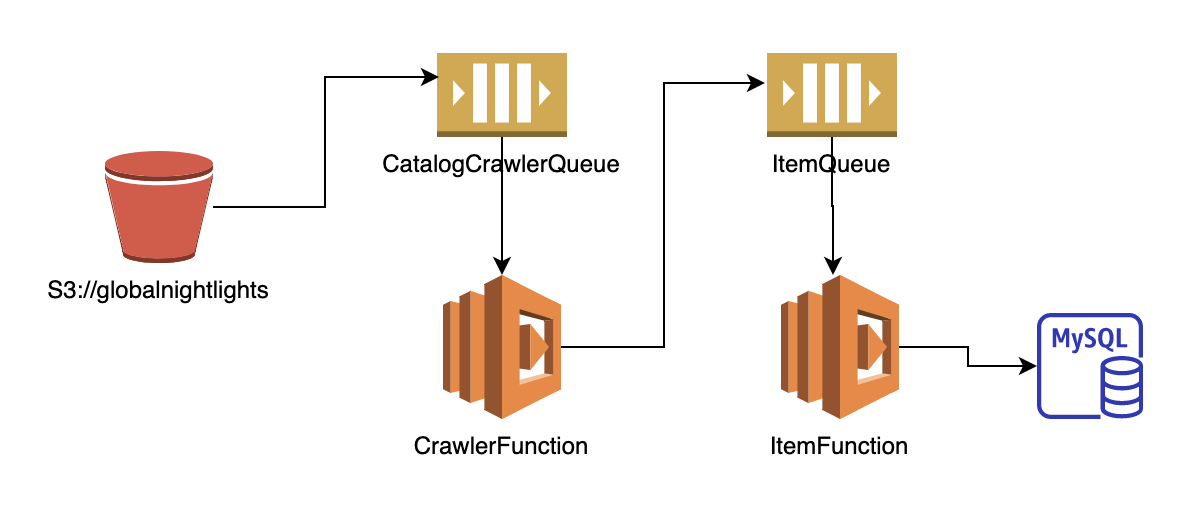
\includegraphics[width=260pt]{images/dataprocess.png}}
		\caption{Data processing}
		\label{fig4}
	\end{figure}
	
	Two Lambda functions are used for processing them, shown as Fig.~\ref{fig4}. The first one is to analyse the STAC protocol files. Boundary box can be found from a STAC file, so it is easy to index
	all the imagery together by it and then to find the specific area by it. Root STAC file is the first file we processing, which has all of the child links as json files. 
	Following the child links, there are the list itmes including the COG file URL. COG file is commonly too large to open directly. GDAL can open it easily and calculate radiance 
	value in the file. In the second Lambda function, messages attached COG URL information exchanged by SQS service from the first Lambda function. Because of the complexity 
	of GDAL computation, the second Lambda function is slower than the first one.
	
	The second Lambda function is the main logic of the data processing. First of all, choosing cities or areas is a deep issue. The original design was to show the every administrative 
	cities. But the global administrative cities geospatial data is very difficult to get. Even though Global Administrative Unit Layers (GAUL) data is provided by Food and 
	Agriculture Organization of the United Nation (FAO) \cite{GlobalAd98:online}, the format of these files still needed to research more. So the research areas were reduced 
	to three specific areas, such as east of China, Middle East and New Zealand. Secondly, these three areas are defined in advance because they represent the areas of developed, 
	developing and war. The radiance of these areas would show very different patterns. And reducing areas can help the function processing more quickly. Thirdly, calculating the 
	radiance for every COG file is the core computation. There are intersection areas between the COG file and these three research places. And every pixel in the COG file stores 
	a radiance value for this geospatial point. In the World Bank document, there are some special definitions about the value details, such as -999.3 means no-data value, -1.5 
	means the beginning of the data range \cite{WorldBan13:online}. The value less than 3 could be disruption value. So all of the numbers which are more than 3 could be the 
	sutiable value. At the end, all of the processed information is stored in RDS service. They are date, boundary box, radiance, pixels and so on.
	
	When it comes to the RDS, it is neccessary to introduce the master and slave configuration. Because this global night lights data is stored at us-east-1 region and team members 
	use ap-southeast-1 region, master database is installed at us-east-1 region which is closed to S3 data, and slave database is at another region. The cross-region RDS is 
	provisioned by CloudFormation because there is a ready template. It has to be mentioned that the cross-region cost is not cheap as other services.
	
	
	\subsection{Testing}
	
	\subsection{Project management}
	Project management is also a big chanllenge in this special period. Scrum development method was chosen from the first day because two of members
	had already experienced this method. This iterative approach towards the completion of a project can lead the team to the success.
	
	It is important that some tools let the team work like a native team. All of the team members are from China, but nobody knew each other before. 
	So at the first day, the IM platform named Lark, which was widely used in the work place in China, was chosen by team members. Java is the first 
	language in the team because team members are almost good at it. By Github, all of the codes can be easily shared with members and easily taken 
	control of its version. Remote cooperation is not a easy thing, so team members create a event for vedio meeting everyday. At the same time, it 
	is also the agile standup meeting everyday. With the development and research process, some members have to stop to learn more things about the 
	lack of relative knowledge. For example, none of members are good at some key technologies, such as geospatial imagery processing, Vue, AWS usage. 
	So the development plan was always disrupted because of the learning. Thanks to the agile method, the development is not influenced too much by 
	these disruptions. 
	
	Because the members were not sharing the true space in a meeting room, the development atmosphere was a little bit strange. It is difficult to know 
	every member's status, so the enthusiasm of development is of critical importance. Somebody went about their tasks with little enthusiasm, and the 
	result would be bad at that aspect. At that time, the role of scrum master was very useful, it ensure the entire development schedule.
	
	\section{Security Considerations}
	Secruity is the important thing in the development. Although some services can enhance the security, but they are usually very expensive, for example, 
	NAT can islote the safer network. There are a lot of details contributing to the security together.
	
	\subsection{IAM}
	
	\subsection{Network}
	
	\subsection{Customer}
	
	
	
	\section{Team members and individual contribution within the team}
	\begin{itemize}
		\item Zhen Chen:  PM, BE, DevOps
		\item Huajie Xu: FE
		\item Shengzhu Wang(Simon): BE
		\item SiXiang Xiong(Tom): BE, Testing
		\item Wenjie Tong: Data Researcher, Testing
	\end{itemize}
	
	
	\subsection{Figures and Tables}
	Use the abbreviation 
	``Fig.~\ref{fig}'', even at the beginning of a sentence.
	
	\begin{table}[htbp]
		\caption{Table Type Styles}
		\begin{center}
			\begin{tabular}{|c|c|c|c|}
				\hline
				\textbf{Table}&\multicolumn{3}{|c|}{\textbf{Table Column Head}} \\
				\cline{2-4} 
				\textbf{Head} & \textbf{\textit{Table column subhead}}& \textbf{\textit{Subhead}}& \textbf{\textit{Subhead}} \\
				\hline
				copy& More table copy$^{\mathrm{a}}$& &  \\
				\hline
				\multicolumn{4}{l}{$^{\mathrm{a}}$Sample of a Table footnote.}
			\end{tabular}
			\label{tab1}
		\end{center}
	\end{table}
	
	\begin{figure}[htbp]
		\centerline{
\includegraphics{fig1.png}}
		\caption{Example of a figure caption.}
		\label{fig}
	\end{figure}
	
	
	
	\printbibliography
	
\end{document}
